%!TEX program = xelatex
% Note: this template must be compiled with XeLaTeX rather than PDFLaTeX
% due to the custom fonts used. The line above should ensure this happens
% automatically, but if it doesn't, your LaTeX editor should have a simple toggle
% to switch to using XeLaTeX.

\documentclass[
  aspectratio=169, % Uncomment to use an aspect ratio of 16:9 (160 mm by 90 mm)
  %aspectratio=43, % Uncomment to use an aspect ratio of 4:3 (128mm by 96mm)
  t, % Top align all slide content by default
  onlytextwidth, % Typeset content in columns at text width
  10pt, % Default font size, use 10pt for the 16:9 aspect ratio and 8pt for the 4:3 aspect ratio
]{beamer}

\usepackage{../../ImperialTheme/beamer/beamerthemeImperial} % Use the Imperial theme

\def\imagefolder{../../ImperialTheme/beamer/Images}
\def\Rey{\text{Re}}
\title{$d=3$ boundary study} % Presentation title to appear on the title slide and left footers

\subtitle{} % Presentation subtitle to appear on the title slide

\author{Víctor Ballester} % Author name(s) to appear on the title slide

\date{\today} % Presentation date to appear on the title slide and right footers

\begin{document}

\begingroup
\setbeamercolor{background canvas}{bg=ICLLightGrey} % Slide background color
\setbeamercolor{title page title}{fg=ICLBlue} % Title text color
\setbeamercolor{title page subtitle}{fg=ICLBlue} % Subtitle text color
\setbeamercolor{author}{fg=ICLBlue} % Author(s) text color
\setbeamercolor{date}{fg=ICLBlue} % Date text color
\setbeamertemplate{title page}[logo]{\imagefolder/ICL_Logo_Blue.pdf} % Imperial logo color, use 'ICL_Logo_White.pdf' for white and 'ICL_Logo_Blue.pdf' for blue
\frame[plain, s]{\titlepage} % Output the title page with no footer ('plain') and vertically distributed text ('s')
\endgroup

\begin{frame}
	\frametitle{Reminder}
	\centering

	\begin{itemize}
		\item Lines $d=2$, $d=1.25$ look correct.
	\end{itemize}

	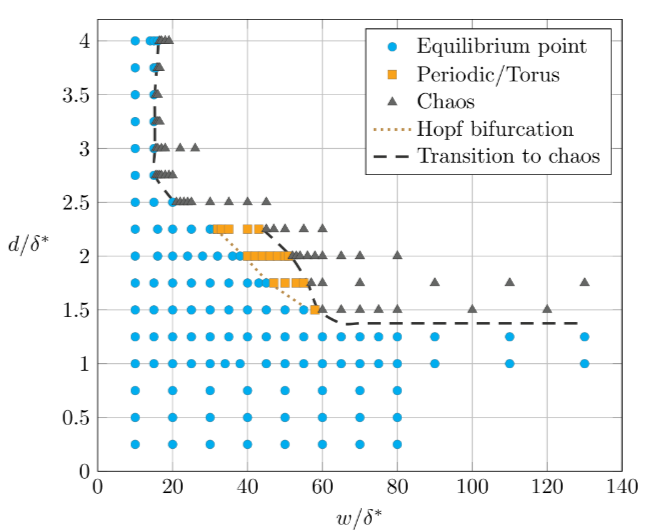
\includegraphics[width=0.5\linewidth]{Images/stabilitycurve.png}
\end{frame}
\begin{frame}
	\frametitle{Sketch of the bifurcation diagram with the info so far}
	\begin{columns}[T] % [T] ensures correct vertical alignment
		\begin{column}{0.69\linewidth} % Left column
			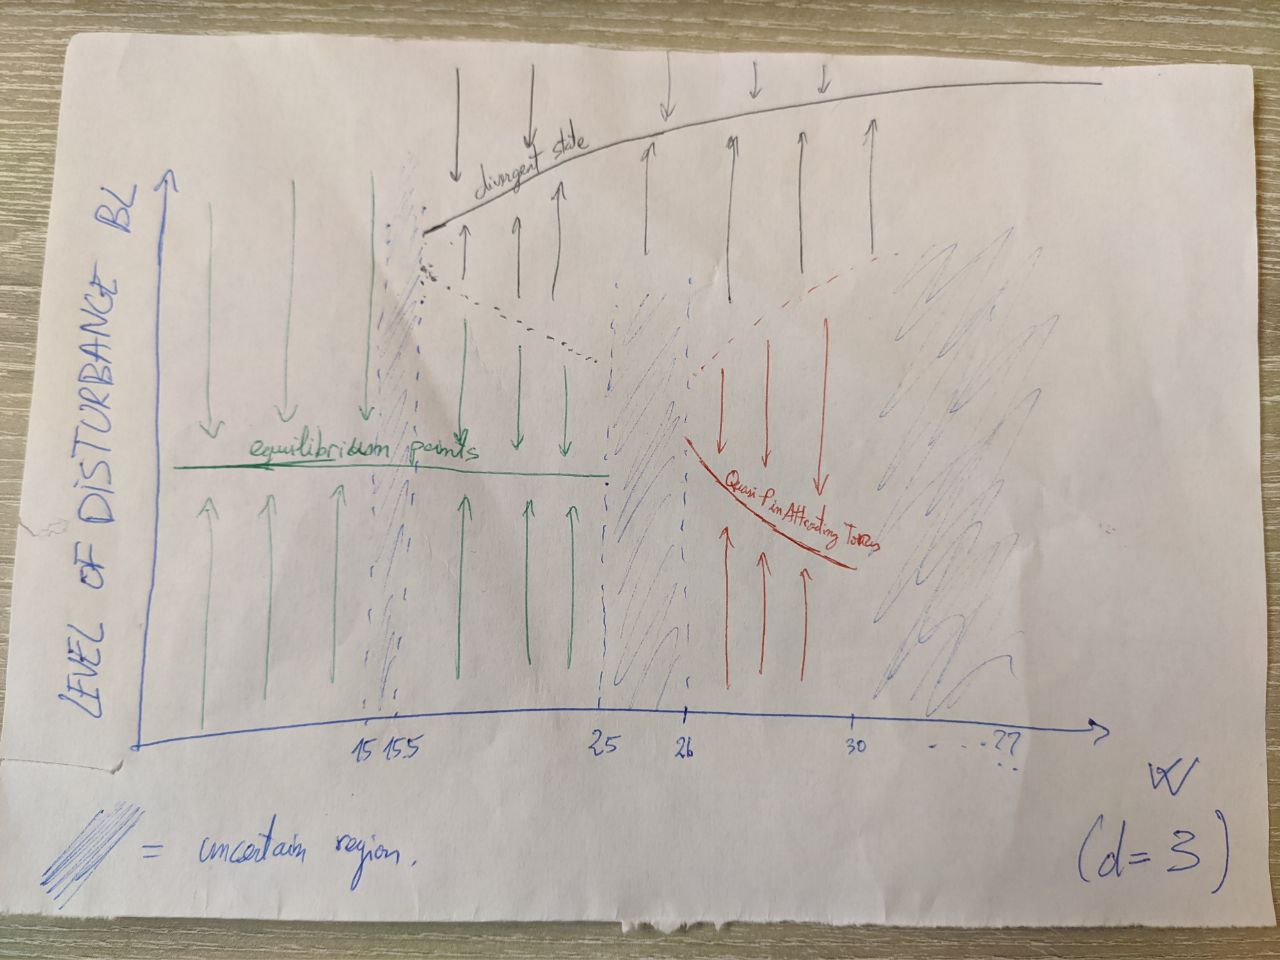
\includegraphics[width=\linewidth]{Images/bifdiagram.jpg}
		\end{column}
		\begin{column}{0.29\linewidth} % Left column
			\begin{itemize}
				\item Bif $w=15.11-15.12$:\\ loss of globally attracting state? 
				\item Bif $w=25.41-25.42$:\\ It is actually a Hopf and what I was obsevring before was the real frequency coupled with a numeric frequency (sampling frequency). There is only one global unstable mode after $w=25.42$.
			\end{itemize}
		\end{column}
	\end{columns}
\end{frame}
\begin{frame}
	\frametitle{$w = 26$ global mode}
	\begin{columns}[T] % [T] ensures correct vertical alignment
		\begin{column}{0.69\linewidth} % Left column
			
\includegraphics[width=\linewidth]{Images/globalmode.png}
			\begin{itemize}
				\item DNS (blue)
				\item $ A e^{\sigma t} \cos(\omega t + \phi)$ (orange),

					$\sigma = 0.0011487$ (growth rate), $\omega = 0.263295$ (frequency).
			\end{itemize}
		\end{column}
		\begin{column}{0.29\linewidth} % Left column
			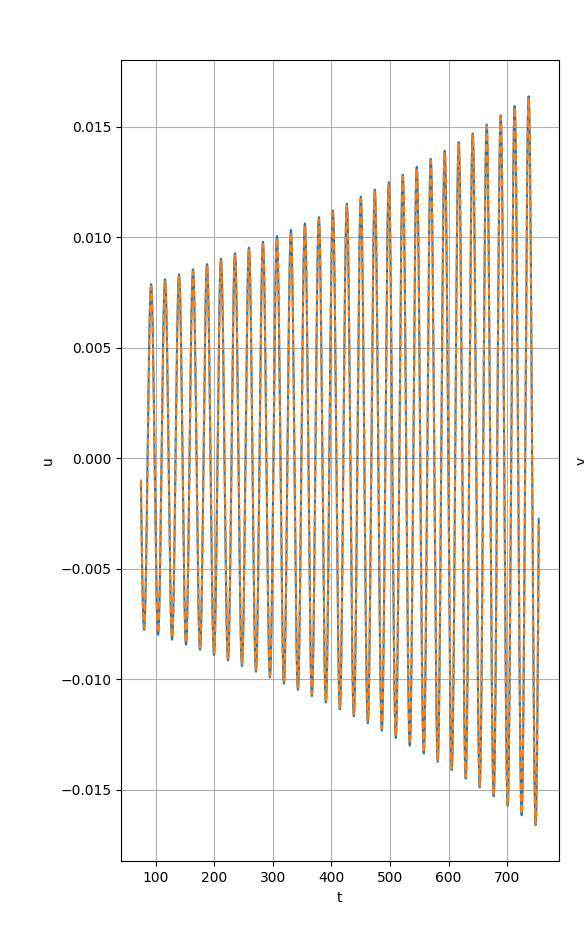
\includegraphics[width=\linewidth]{Images/prediction.png}
		\end{column}
	\end{columns}
\end{frame}
\end{document}
